% =============================================================================================
% 1 Introduction (problem formulation + related work)
% Numbers: 实验结果汇总.md (5-repeat run, 2026-10-24); literature: litreview/abstracts.md
% =============================================================================================
\section{Introduction}
\label{sec:intro}

\paragraph{The clinical problem.}
Hip osteoarthritis (OA) has no single diagnostic standard. The clinical criteria of the American College of Rheumatology
rest on hip pain, restricted internal rotation and morning stiffness~\cite{altman1991acr}; NICE allows a diagnosis without
imaging~\cite{nice2022oa}; epidemiology relies on the radiographic Kellgren--Lawrence (KL) grade and the OARSI atlas
items~\cite{altman2007oarsi}. The three often disagree: among early symptomatic patients, radiographic OA is almost as
common in painless as in painful hips~\cite{rondas2022}. For the end stage, total hip arthroplasty (THA) is
effective, and implants now last: about 58\% of hip replacements still function after 25 years~\cite{evans2019hip}.
This shifts the clinical question for the 45--65-year-old patient. Every year of joint survival counts, because a younger
recipient carries a higher lifetime risk of revision~\cite{bayliss2017revision}. What guides the intensity of conservative
care, the timing of orthopaedic referral and the enrolment in joint-preserving trials is therefore a \emph{long-horizon}
estimate of whether, and roughly when, this hip will need replacing.

\paragraph{What AI prediction offers so far.}
Prediction work in OA is dominated by the knee, and the hip makes up only 8--15\% of OA--AI studies~\cite{binvignat2022}.
Most hip models classify the current KL grade or predict incident radiographic OA. Only one large study predicts THA
from pixels: in the Osteoarthritis Initiative (OAI) a model with deep-learning radiographic measurements reached AUROC
0.81 and AUPRC 0.28 for 10-year THA at a 2.4\% event rate~\cite{jang2023}. External validation remains rare. When it is
done, performance falls; for example, a seven-cohort hip model dropped from AUROC 0.81 to 0.64 under leave-one-cohort-out
validation~\cite{vandenberg2026}. Table~\ref{tab:forest} summarises the prognostic literature. The \textbf{Cohort Hip and
Cohort Knee (CHECK) study} is the natural test bed for the surgical question~\cite{wesseling2016}. Between 2002 and 2005,
ten Dutch hospitals enrolled 1,002 people aged 45--65 with hip or knee pain, at or within six months of their first
general-practitioner visit for these symptoms; participants were referred by general practitioners or responded to
advertisements. They were followed for ten years with
questionnaires, standardised examination and radiographs. In our analysis this gives 2,004 hips; 1,705 have known 10-year
status, and 93 (5.5\%, in 75 people) were replaced. We use every baseline item that is fixed at first presentation: 76
clinical features in six groups and the pixels of the baseline anteroposterior (AP) pelvic radiograph. Linear, tree and
FT-Transformer models handle the tables. A supervised residual head on frozen DenseNet features turns the pixels into a
single risk score, and an elastic net fuses the two.

\begin{table}[!tbp]
  \centering
  \caption{\textbf{Prognostic models for hip (and, for reference, knee) OA: cohort, event rate and performance.}
  Left: discrimination (AUROC; solid bars = reported 95\% CI, dashed = Hanley--McNeil interval from hips and events, or
  $\pm$SD across held-out cohorts; marker area $\propto\log$ events). Right: AUPRC divided by the event rate, the only
  scale on which precision is comparable across cohorts; studies that do not report the event rate show the raw AUPRC.
  Colours give the model input. Endpoints differ (THA, radiographic OA (rHOA), KL progression), so no pooled estimate is
  drawn. Our rows (grey band) are nested cross-validation means; CIs from a participant-clustered bootstrap. Agricola
  2013 reports apparent performance (shape modes selected and evaluated on the same data).}
  \label{tab:forest}
  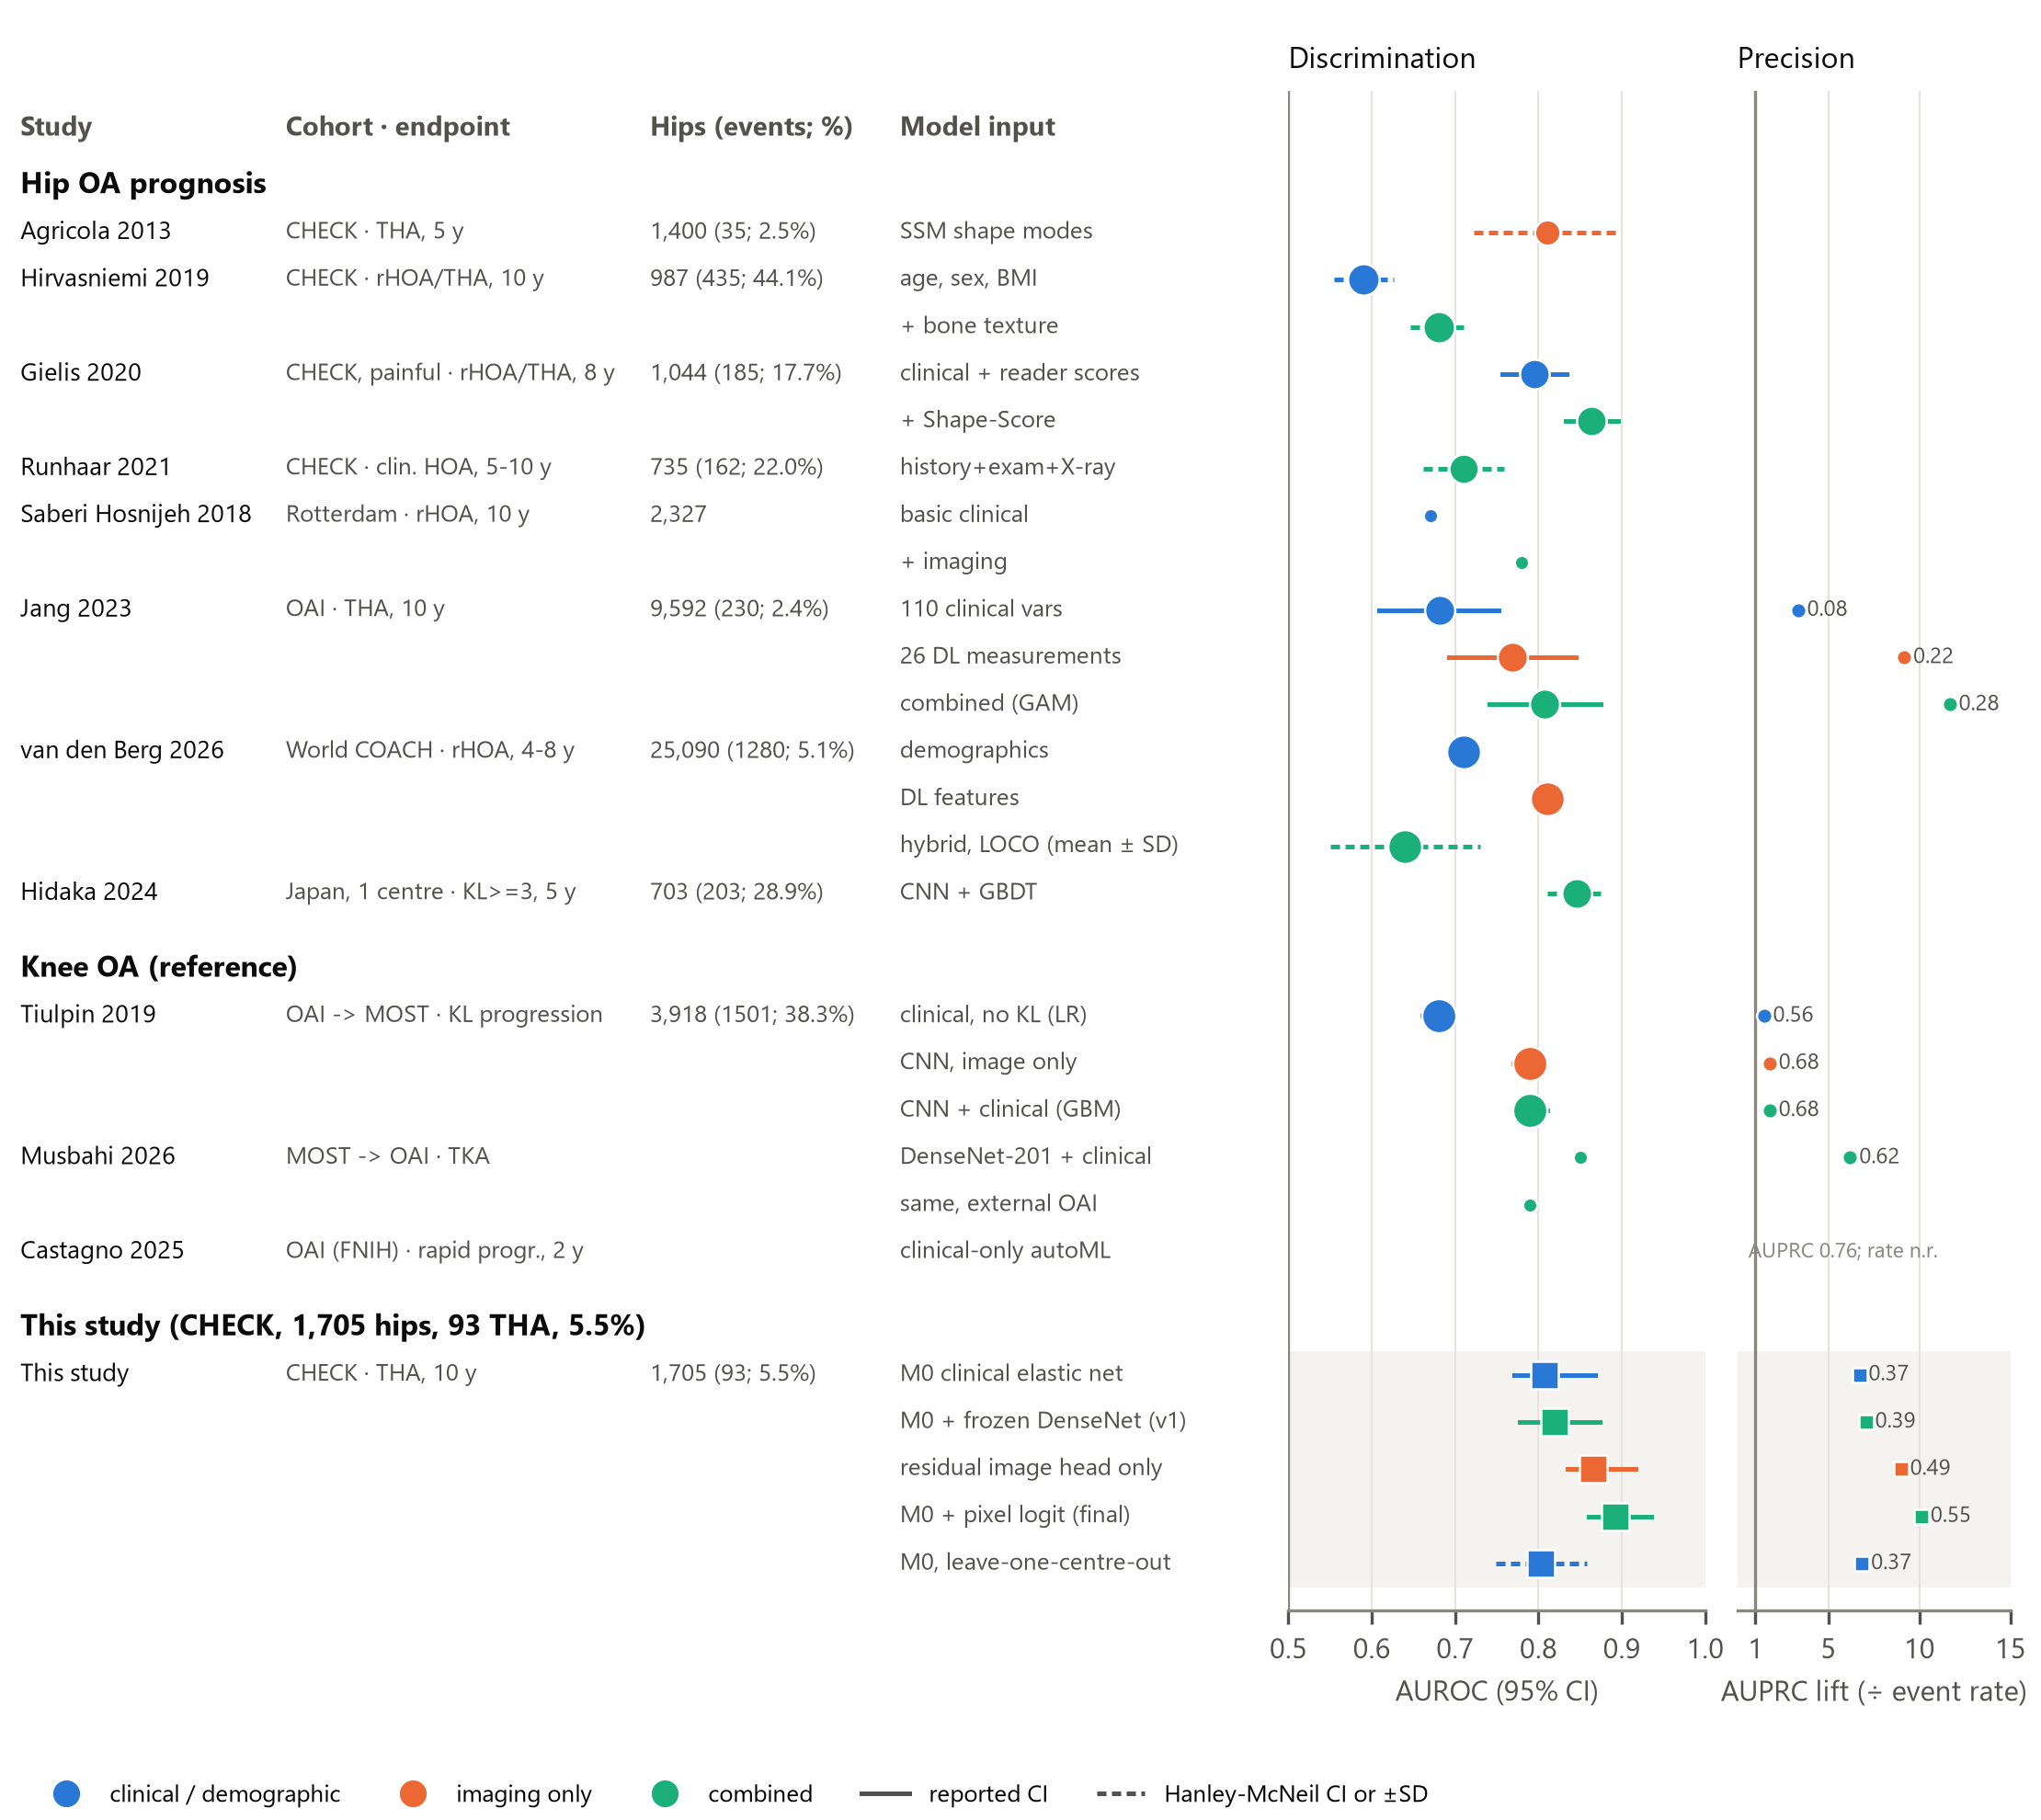
\includegraphics[width=\linewidth]{tab1_forest.png}
\end{table}

\paragraph{Prior work on CHECK and on the knee.}
Hip models built on CHECK share a pattern~(Table~\ref{tab:forest}). The image enters as hand-crafted structure:
statistical shape modes predict 5-year THA (AUROC 0.81, 35 events)~\cite{agricola2013}, an automated Shape-Score raises
8-year radiographic OA prediction from 0.795 to 0.864~\cite{gielis2020}, and bone texture adds 0.09 to a demographic
model~\cite{hirvasniemi2019}. The endpoints are mostly radiographic. Several models also contain the baseline KL grade,
which in the public CHECK release was read after follow-up, paired with later films~\cite{macri2022}. Clinical-only
predictors are weak for radiographic outcomes~\cite{saberihosnijeh2018,vanberkel2021}. For arthroplasty, however,
symptoms (WOMAC), age and sex are the established predictors~\cite{zarringam2020}. The surgical endpoint is thus where
non-imaging information should be given importance.

\paragraph{}
Knee studies show what changes with anatomy and endpoint. On standing knee films the joint space is seen directly,
without pelvic overlap, and the outcome (KL progression) is itself read from the film. So an end-to-end CNN with a KL
auxiliary task beats clinical data (0.79 vs 0.68)~\cite{tiulpin2019}. For surgery, a DenseNet with clinical inputs
reaches 0.85 internally and 0.79 externally~\cite{musbahi2026}. Clinical-only models transport well~\cite{castagno2025}.
A systematic review of 33 deep-learning studies found that combining imaging modalities did not consistently help, that
external validation lowered the median AUC from 0.81 to 0.75, and that surgical endpoints also reflect access to
care~\cite{gillani2026}. The hip joint is deep,
small on a pelvic film, and partly hidden by the acetabular rim. Its early signs (superolateral joint-space narrowing,
marginal osteophytes) are millimetre-scale and local. A frozen, globally pooled ImageNet embedding is therefore unlikely
to capture them.

\paragraph{Connection to the course.}
Our image baseline follows the frozen-feature-extractor approach of Bar et al.\ (Lecture 2, slides 102 and 126--127;
video 1:00--1:05). The decision to freeze rather than fine-tune follows the transfer-learning guidance for scarce
labelled data (Lecture 2, slides 106--114; video 0:54--0:56). DenseNet-121 is the CheXNet backbone, whose saliency maps
motivated our attention maps (Lecture 2, slide 158; video 1:29--1:31). Class-weighted losses for imbalance follow
Lecture 3 (slides 63--64; video 0:31--0:34). Our token, FiLM and logit fusions map onto the early, joint and late fusion
types of Lecture 8 (slide 30; video 0:11--0:14), and our SimCLR pretraining onto its self-supervision section (slides
42--50; video 0:17--0:20). Appendix~\ref{app:lectures} lists all links.

\paragraph{}
Our design follows from these observations. (i) With 93 events and 76 features (about 1.2 events per feature), a
penalised linear model is the reference that every deep model must beat~\cite{christodoulou2019}. (ii) The image head
keeps the $14\times14$ spatial map of a frozen DenseNet-121 and adds two residual blocks with attention pooling. Its
features are supervised with the 11 OARSI reading items, used \emph{only as training targets}, so the future-informed
readings never become predictors. (iii) The image enters the clinical model as one cross-fitted logit, a learned
analogue of Jang's measurements~\cite{jang2023}, because token fusion overfits at this sample size. (iv) No external
cohort with the same inputs was available. Every estimate is therefore internal (nested cross-validation within CHECK),
and transportability is probed with pseudo-external splits across centres, film formats and patient subgroups rather
than claimed.

\paragraph{Research question and clinical setting.}
We fix the prediction time $t_0$ at the first consultation for hip or knee complaints, when the AP pelvic radiograph is
taken. The question is: \emph{from history, questionnaires, a standardised hip examination and the raw pixels of that
same-day radiograph (with no radiologist's grading and no research biomarkers), what is this hip's risk of replacement
within ten years?} The intended uses are deciding how intensive conservative management should be and how often to
review, timing the referral to an orthopaedic surgeon, and enriching joint-preservation trials with high-risk hips. Two
uses are excluded. Hips that are already on a surgical pathway at $t_0$ gain nothing from prediction. Population-level
planning is also out of scope without local recalibration (Section~\ref{sec:res-aux}). We ask four things:
\begin{enumerate}[leftmargin=*,itemsep=0pt,topsep=2pt]
  \item How much do examination and symptoms add beyond demographics?
  \item Does a deep tabular model outperform a penalised linear model?
  \item Can radiographic signal be extracted from pixels alone, without readings at prediction time?
  \item Do discrimination and calibration transport across centres, film formats and patient subgroups?
\end{enumerate}
Figure~\ref{fig:overview} summarises the inputs, models and outputs of the study.

\begin{figure}[!tbp]
  \centering
  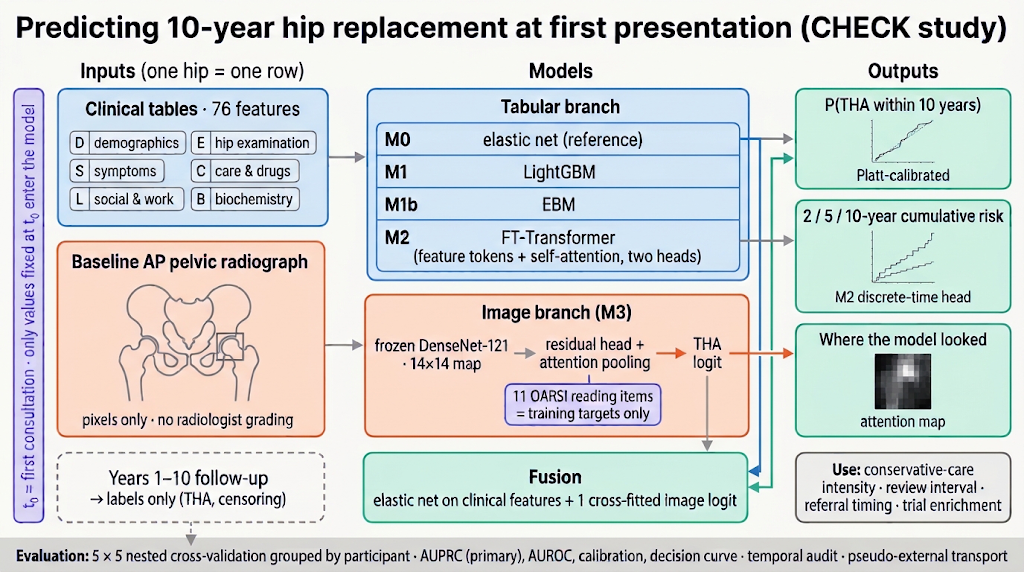
\includegraphics[width=\linewidth]{fig1_overview.png}
  \caption{\textbf{Inputs, models and outputs.} Baseline clinical tables (76 features, groups D/E/S/C/L/B) and the
  baseline AP pelvic film are the only inputs. The tabular branch compares a penalised linear model with tree ensembles
  and an FT-Transformer. The image branch converts each hip crop into one THA logit. The final model is an elastic net on
  clinical features plus that logit. Outputs are the Platt-calibrated 10-year THA probability and, from the
  FT-Transformer's discrete-time head, 2/5/10-year cumulative risk.}
  \label{fig:overview}
\end{figure}
